\section{Evaluation}

We implemented a prototype of the follow-up question selection of the \evpi system (i.e., Offline Corpus Curation and Selecting Follow-Up Questions, as shown in Figure~\ref{fig:pipeline}) with the aim of evaluating its combined efficacy along
a few different dimensions. First, we use metrics and a held-out data set to evaluate the quality
of the recommendation, i.e., how well the system selects valid follow-up questions for incomplete bug reports. We define {\em valid} follow-up questions as those that are a match to the topic and content of a specific bug report.
Second, we use a survey of software developers to evaluate the follow-up questions on their usefulness, novelty and specificity. We define {\em usefulness} as the perceived ability of the follow-up question to elicit additional valuable information for diagnosing the bug; {\em novelty} as the perceived ability to elicit new, previously unreported information, and {\em specificity} as how much the follow-up question is tailored for the target bug report vs. applicable to a broad range of other bug reports.

\begin{figure}
	\centering
	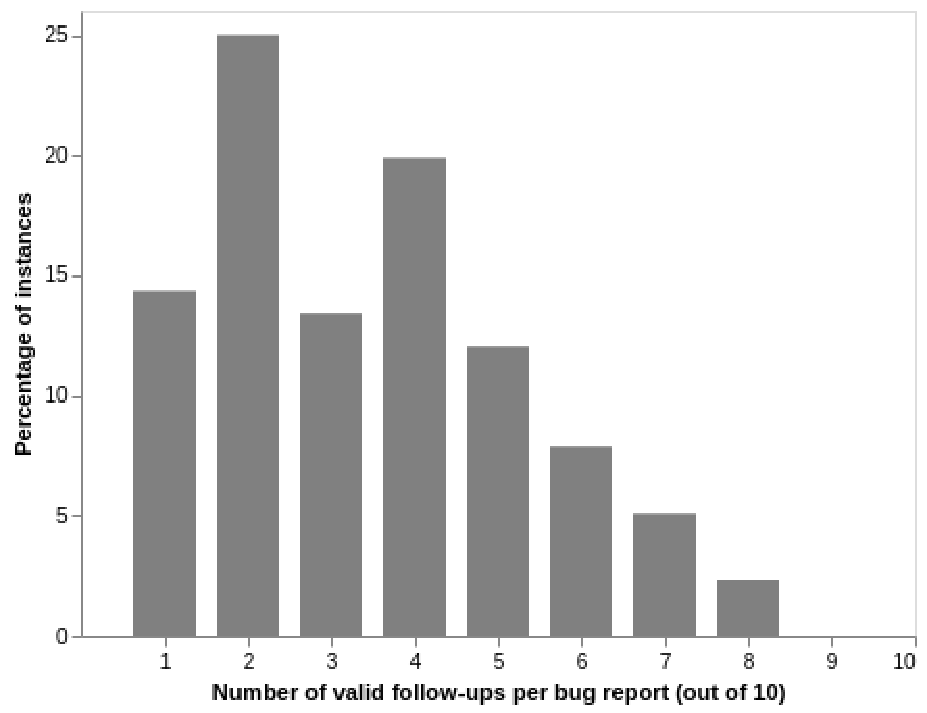
\includegraphics[width=0.8\linewidth]{figures/viz_annotation.pdf}
	\caption{Distribution of valid follow-up questions in the held-out set (average=3.45).}
	\label{fig:annotation}
\end{figure}

\newcommand*{\tab}{\hspace*{0.5cm}}%

\begin{table*}[t]
\centering
\caption{Evaluation results contrasting our system (\evpi) relative to several baselines.}
\begin{tabular}{|p{3cm}|ccc|ccc|ccc|ccc|}
\hline
%                          & \multicolumn{4}{c}{$V_{1} \cap V_{2}$} \\\hline
& \multirow{2}{*}{\bf MRR} & Wilcoxon & Effect & \multirow{2}{*}{\bf P@1} & Wilcoxon & Effect & \multirow{2}{*}{\bf P@3} & Wilcoxon & Effect & \multirow{2}{*}{\bf P@5} & Wilcoxon & Effect \\
&                          & $p$-value & size   &                          & $p$-value  & size   &                          & $p$-value  & size   &                          & $p$-value  & size \\ \hline
{\em \evpi}               & {\bf 0.677} & - & - & {\bf 0.486} & - & - & {\bf 0.492} & - & - & {\bf 0.446} & - & - \\ \hline
{\sc Baselines:}   &  &  &  &  &  &  &  &  &  &  &  &  \\ 
\tab {\em Random}              & 0.542 & $p$ $<$ 0.01 & 0.229 & 0.319 & $p$ $<$ 0.01 & 0.167 & 0.368 & $p$ $<$ 0.01 & 0.216 & 0.355 & $p$ $<$ 0.01 & 0.214 \\
\tab {\em Lucene}              & 0.534 & $p$ $<$ 0.01 & 0.252 & 0.347 & $p$ $<$ 0.01 & 0.139 & 0.318 & $p$ $<$ 0.01 & 0.308 & 0.317 & $p$ $<$ 0.01 & 0.294 \\
\tab {\em Rao et al.~\cite{rao-daume-iii-2018-learning}}  		  & 0.551 & $p$ $<$ 0.01 & 0.218 & 0.342 & $p$ $<$ 0.01	& 0.144	& 0.336 & $p$ $<$ 0.01 & 0.279 & 0.342 & $p$ $<$ 0.01 & 0.245 \\
\tab {\em Utility only}        & 0.646 & $p$ = 0.11   & 0.059 & 0.468 & $p$ = 0.60   & 0.019 & 0.443 & $p$ = 0.01   & 0.087 & 0.412 & $p$ = 0.01   & 0.077 \\
\tab {\em Compatibility only}  & 0.612 & $p$ = 0.01   & 0.115 & 0.426 & $p$ = 0.11   & 0.060 & 0.383 & $p$ $<$ 0.01 & 0.196 & 0.377 & $p$ $<$ 0.01 & 0.152 \\ \hline
\end{tabular}
\label{tab:results}
\end{table*}


\subsection{Quality of Follow-Up Question Ranking}

One way of evaluating the ranking system, based on a held-out dataset (of bug reports and candidate follow-up questions), is
by using the posed questions as the ground truth. However, this simple setup has a serious deficiency in that the actually posed question
may not always be the most optimal among the set of candidate follow-up questions. More importantly, several of
the remaining candidate questions may be valid and (more) relevant to the bug report and therefore should
not be considered as negatively labeled instances for evaluation. Therefore, in order to provide an evaluation
set that identifies all of the valid questions in the candidate set, we perform manual annotation that clearly
identifies all of the valid follow-up questions for a specific bug report.



\subsubsection{Annotation}
We annotated 400 randomly chosen bug reports that were held-out from training in our original corpus of 25K (curated as described in Section~\ref{sec:select_corpus}). The annotation
was performed by two of the authors following an agreed-upon predefined procedure. We focused our annotation on the 10 candidate follow-up question retrieved by Lucene. For each bug report, each annotator 1)
read the bug report carefully, spending a few minutes to understand its context, e.g., by looking at the purpose of the overall GitHub
project and the types of technologies it relies on; 2) marked all of the follow-up questions for the candidate set of 10
that were valid. Both of the annotators processed the same set of 400 bug reports, marking an average of 3.45/10 of the follow-up questions as valid with an inter-annotator agreement (Cohen's kappa) of 0.60. The distribution of valid follow-up questions is shown in Figure~\ref{fig:annotation}.
We use the set of follow-up questions that both annotators agreed were valid, i.e., the intersection between their annotations.



\subsubsection{Baselines}
The baselines we identified are meant to convey both straightforward approaches to ranking (e.g., directly using the Lucene output) and
ablation, i.e., using one part of our ranking function but not the other (e.g., ranking based only on the question utility, $U(q_{i})$).
We did not find directly related prior techniques to compare against, since the research direction is novel and models from other domains
with a similar purpose are too different in form. Below is an enumerated list of all of the ranking baselines we used.
\begin{itemize}
\item {\em Random} -- A random permutation of the candidate follow-up question list. We present metrics averaged over 10 runs.
\item {\em Lucene} -- Lucene uses the vector space model (i.e., {\em tf*idf}) to rank follow-up questions based on the similarity between the bug reports. This baseline just transfers Lucene's ranking, which we use to generate our candidate set of 10 follow-up questions, as the system's output.
\item {\em Utility only} -- $U(q_{i})$ -- The utility function, described in detail in Section~\ref{sec:ranking}, computes the average amount of OB, EB or S2R found in the answers to the specific follow-up question.
\item {\em Compatibility only} -- $P(q_{i}+a_{i}|br)$ -- The compatibility function computes the probability a bug report can be combined with a specific follow-up question and answer pair. The implementation uses a deep NN architecture to compute this value.
\end{itemize}

\subsubsection{Metrics}
We use two popular information retrieval evaluation metrics: Mean Reciprocal Rank (MRR) and Precision@n (P@n).

The goal of MRR is to evaluate how effective is our technique, or a baseline, in locating the first valid follow-up question, as, presumably, this is a proxy for the ease with which an end-user would locate a follow-up question in the ranking. It is
computed as: $$MRR = \frac{1}{|B|} \sum_{i=1}^{|B|} \frac{1}{rank_{i}}$$ ,where $B$ is the set of bug reports in the test set and $rank_{i}$ is the ranked position of the first valid follow-up question for the $i^{th}$ bug report.

The goal of Precision@n is to measure the number of valid results when considering the top $n$ positions in the ranking. Unlike MRR, it consider all, not only the topmost ranked, results. It is computed as: $$P@n = \frac{1}{|B|} \sum_{i=1}^{|B|} \frac{|v|}{n}$$ ,where, as before, $B$ is the set of bug reports in the test set and $v$ is the set of valid follow-up questions ranked in the top $n$ positions. We use values of 1, 3 and 5 for $n$.

We compute Wilcoxon's signed rank test for each of the above metrics to estimate the statistical significance of the difference between our technique \evpi and the baselines. The effect size of the comparison is calculated using Cliff's delta ($\delta$) ~\cite{cliff1993dominance}, which ranges from -1 (all values in the first group are larger than the second group) to +1 (all values in the second group are larger than the first group). A value of zero indicates that the two groups are identical. The criteria for interpreting $\delta$ is that $|\delta| >$ 0.147 $\rightarrow$ small effect, $|\delta| >$ 0.33 $\rightarrow$ medium effect, and $|\delta| >$ 0.474 $\rightarrow$ large effect ~\cite{romano2006appropriate}.

\begin{figure*}[t]
\centering
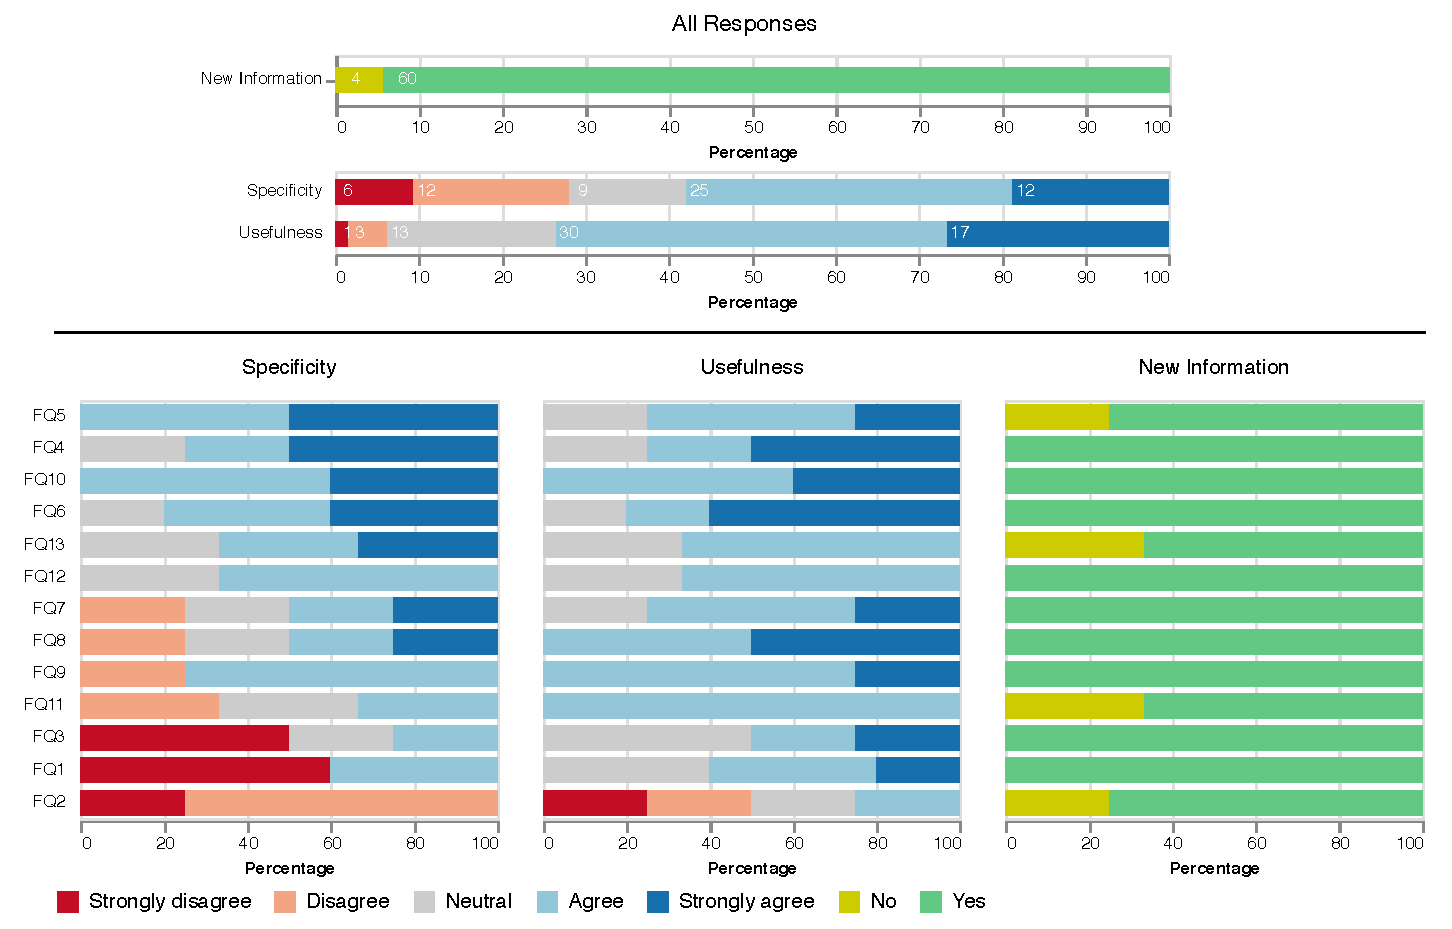
\includegraphics[width=0.95\linewidth]{figures/viz_group.pdf}
\caption{Responses to developer survey grouped per category (top) and per follow-up question (bottom). FQ$n$ = Follow-Up Question $n$.}
\label{fig:survey}
\end{figure*}

\subsubsection{Results}
We summarize the results of our technique (\evpi) versus the identified
baselines in Table~\ref{tab:results}. Our results indicate that \evpi outperforms all of the baselines,
with the ablation-type baselines performing better than the simple baselines. The Lucene ranking
does surprisingly poor, basically in line with the Random baseline. The Utility only baseline is
the ones that comes closest to the performance of the full system. Perhaps the most intuitive result
is $P@1$, where \evpi scores 0.49, indicating that just about half of all of the top selected follow-up
questions by our system were valid. The Wilcoxon's signed rank test and the Cliff's delta confirm the observations from
the raw metric values, i.e., that Utility only has a strong similarity to \evpi and could be strong contributing
factor to the approach's effectiveness. They also confirm that \evpi has a strong advantage over the simple
baselines.

We interpret the results 

\begin{table*}[t]
	\centering
	\caption{Comparison of the \evpi follow-up question and the actually posed (original) follow-up question for three of the highest rated instances by the survey respondents.}
	\begin{tabular}{ |M{1cm}|p{7.3cm}|p{4cm}|p{4cm}|  }		\hline
		% Instance &Bug report & Bug-IQ follow-up question & Original follow-up question\\		\hline
		% FQ9
		% & {\em Title =} "random.multivariate\_normal broken in python 3" \newline
		% {\em Body =} "The following example [...] \newline
		% gives [...] in python-2.7.11 \newline
		% and [...] in python-3.4.4 both with numpy 1.10.2."
		% & Could you try upgrading/re-installing your numpy? \newline
		% (Also refer - [this SO answer] (http://stackoverflow.com/[...]))
		% & How did you install numpy? What platform are you on? If you installed numpy yourself, you might want to check that you have made a clean install.		\\ \hline

		FQ22
		&{\em Title =} "Plugin is not working on latest android" \newline
		{\em Body =} "On app start: [...] \newline
		On Button Click: [...] \newline
		I am running the example code on Arch Linux with Java 8, latest Android SDK with target API 22 and default nexus 5 ADM Config.
		Any ideas why the SpeechRecognition object is not being initialized?""
		& [...] Are you waiting for the device ready to fire before calling the SpeechRecognition?
		& [...] Are you waiting for the device ready to fire before calling the SpeechRecognition?\\ \hline

		FQ14
		&{\em Title =} "Multiple time tests discovering" \newline
		{\em Body =} "I have strange problem with running xunit tests as part of my build process. Since yesterday after running all tests my tfs build starts discovering tests again and after that it runs tests again. And that's repeated 15 times.
		Below I have log from TFS: [...]"
		& Can you describe your scenario a little more? One way of doing this is described in [...]
		& Can you check if you have multiple copies of the xUnit adapter under [...]? Thanks! \\ \hline
	\end{tabular}
\label{tab:survey}
\end{table*}


\subsection{Developer Survey}
While a recommended follow-up question may be valid, it may not possess other properties that would
encourage its use in practice, i.e., in a system that automatically poses follow-up questions for incomplete bug reports. For
instance, a follow-up question may be overly generic, lacking detail or context specific to the bug report (e.g., {\em Can you provide
additional information?}). To investigate how \evpi performs across several such dimensions of interest we conducted a survey with
software developers.

%\subsubsection{Participants}
Through personal contacts, we e-mailed 10 software developers about the study, providing the basic context of our project
and a link to a Web form containing the survey. None of the developers were
aware about the details of our technique. The developers were half (5) from academia (graduate students at
institutions in the U.S. and Europe) and half professional developers from industry. All had programming
experience of 4 or more years with popular languages like Java and Python and all indicated one of their primary
responsibilities was developing software.

%Procedure
We randomly assigned the developers into two groups of 5 and each group was assigned 12 instances of bug report and follow-up question pairs, where all of the follow-up questions were the top-1 selected by \evpi. Each group was presented with bug reports from our corpus that belong to GitHub projects where Java or Python are the primary technologies. For each of the assigned bug reports, a developer
was presented with a screenshot from GitHub containing the title and text of the bug report, the follow-up question, and a link to the project the bug report came from for context. Prior to beginning the survey, we gave instructions to the developers to read both the bug report and the follow-up question before answering the provided set of survey questions. A preliminary survey question, which was posed on an initial screen, asked {\em Is the follow-up question valid?}. A negative response indicated that the follow-up question was invalid and unusable, therefore we asked no additional questions for that specific bug report - follow-up question pair. The remaining survey questions only appeared for instances deemed valid by a developer.

%Measures
For a valid follow-up question, we posed a yes/no survey question asking {\em Does the follow-up question ask for new information currently not included in the description?}, followed by two Likert score survey questions (5 point; Strongly Disagree, Disagree, Neutral, Agree, Strongly Agree) interrogating whether {\em The follow-up question is specific to the bug report} and {\em The follow-up question is useful to the bug report}. In the following, we refer to the first (yes/no) survey question as measuring New Information, the second measuring Specificity, and the third measuring Usefulness.

%Results
The survey results showed that out of the 24 different bug report - follow-up question pairs, a majority of participants (at least 3 out of 5) considered 13 follow-up questions as valid, and 11 as invalid. This ratio is analogous to the results we observed for Precision@1 in the held-out set evaluation presented above, confirming our expectations.

The results of the survey, along each dimension, are presented both at the granularity of an individual response and at the granularity of a bug report (and follow-up question pair) in Figure~\ref{fig:survey}. The survey results indicate that among the categories of Usefulness, Specificity, and New Information, the follow-up questions selected by \evpi provide the most of New Information, followed by Usefulness and Specificity. However, all three categories were generally positive with over 50\% of all responses on each either agreeing or strongly agreeing with the statements on Specificity and Usefulness or affirming that the follow-up question was asking for New Information. Considering the data per follow-up question, in the bottom part of Figure~\ref{fig:survey}, we observe most follow-up questions, which were deemed as valid, were rated positively.  Some follow-up questions have strongly positive ratings, e.g., follow-up question 14 (FQ14) was rated by all 5 respondents as valid, 4/5 agreeing or strongly agreeing that the question was specific, 4/5 agreeing or strongly agreeing that the question was useful, and 5/5 agreeing that the question aimed to provide new information for the bug report.

To further illustrate \evpi's performance, we contrast the \evpi follow-up questions to the ones posed in the original bug report for three of the highest rated survey instances in Table~\ref{tab:survey}. While for one of the instances, FQ22, the recommended follow-up question matches the posed follow-up question, which is possible since the original follow-up question is among our candidate set, the follow-up question in FQ15 is different, asking the question of {\em Can you describe your scenario a little more?} and providing some additional context on how to do so in the succeeding sentence. {\bf ADD FQ8}


% \evpi's follow-up question in FQ9 is specific to {\em numpy}, which is a library mentioned in the bug report, while FQ14 asks the question of {\em Can you describe your scenario a little more?} and provides some additional context in the succeeding sentence.


\subsection{Threats to Validity}
The presented approach is affected by several limitations that may negatively impact the validity of our findings and their ability to generalize. In this section, we discuss those threats as well as strategies we have undertaken to mitigate them.

\noindent{\em Construct validity.}
One threat to construct validity is our use of a manually annotated dataset for the held-out dataset evaluation. We limited this threat by following an annotation process that required the annotators to get familiar with each project. We also observed reasonable Cohen's Kappa values between the two annotators.

A threat to construct validity is also in the preprocessing of bug reports, since we focus only on the textual content of an issue and ignore other enclosed types of information, such as images or links. As a result, for some deficient bug reports, our technique may miss potentially relevant information to locate the most useful follow-up questions. This threat is partially mitigated by the size of the corpus, containing 25K GitHub issues with various characteristics and content.

The notion of utility of a follow-up question poses another threat to validity, since it is based only on a subset of information that can be enclosed in a bug report. To mitigate this threat and select the most useful type of information, we followed prior studies that reported S2R, OB and EB among the most helpful categories of information according to software developers~\cite{Zimmermann2010}.

%Furthermore,  combining OB, EB ans S2R in the utility function lead to another threat...


\noindent{\em Internal validity.}
The limited number of follow-up questions associated with each bug report poses a threat to internal validity. Each bug report is assigned 10 candidate question to rank, instead of processing the whole corpus of available questions. This  may lead to omitting follow-up questions that are valid and specific in the context of a particular bug. We partially mitigate this threat by selecting the most similar bug reports, while also extending the content of each bug report with the bug's labels and repository tags in order to provide Lucene with contextual information that can be leveraged when locating similar issues.


\noindent{\em External validity.}
In this study, we leveraged a dataset of 25K GitHub issues, however, during evaluation we use a subset of 400 manually annotated bug reports. The limited size of the test set may impact our observations as it covers only a small subset of population. To mitigate that threat, we include bug reports from 357 open-source software projects leveraging different frameworks and technologies. Moreover, to ensure the quality of the proposed approach, we conducted a user study with 10 software developers. We observed that the number of valid follow-up questions in the user study nearly matched the result obtained in the held-out evaluation, emphasizing the overall quality of the system and supporting validity of the results.

The scope of the developer survey poses another threat to external validity due to the low number of enclosed bug reports and selection of issues only from Python or Java-related software projects. We partially mitigate bias caused by limiting the bug reports to only two technologies by sampling issues with different content characteristics (e.g., with or without stack traces) from multiple projects.  To ensure the quality and generalizability of the survey results, each pair of bug report and follow-up question was assessed by half of the respondents.
